% siminos/atlas/cut.tex  pdflatex atlas
% $Author$ $Date$

\section{Sections}
\label{s:cut}

In the {\em Poincar\'e section} method one records the coordinates of the
trajectory $\ssp(\zeit)$ at the instant, $\sspRed_n = \ssp(\zeit_n) \in
\PoincS$, it traverses an oriented fixed hypersurface $\PoincS$ of
codimension 1. For high-dimensional flows that we have in mind, the only
feasible section is a hyperplane, the type of Poincar\'e section (or,
from now on, just a \emph{section})  we shall consider here. Such a
section captures important features of the flow in an open neighborhood
of the section-fixing \template.

%%%%%%%%%%%%%%%%%%%%%%%%%%%%%%%%%%%%%%%%%%%%%%%%%%%%%%%%%%%%%%%%%%%%%
\begin{figure}
  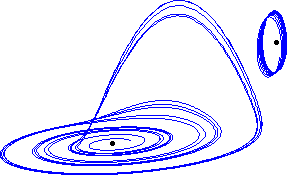
\includegraphics[width=0.3\textwidth]{RoessTrjs}
    \caption{
R\"ossler \eqva\ and their invariant manifolds. The stable manifold of
the inner {\eqv} $\ssp_{-}$  is 1-dimensional and the unstable one is a
spiral-out focus. For the outer {\eqv} $\ssp_{+}$  the stable manifold is
a spiral-in focus (basin boundary for initial conditions that either fall
into the chaotic attractor, or escape to infinity) and the unstable
manifold is 1-dimensional.
    }
\label{fig:RoessTrjs}
\end{figure}
%%%%%%%%%%%%%%%%%%%%%%%%%%%%%%%%%%%%%%%%%%%%%%%%%%%%%%%%%%%%%%%%%%%%%

As an example consider the system of R\"ossler\rf{ross},
\index{R\"ossler system}
\beq
\begin{split}
  \dot{x} &= -y \,-\,z \\
  \dot{y} &= x + a y \\
  \dot{z} &= b + z (x - c)
  \,,
  \label{eq:Rossler}
\end{split}
\eeq
where $a = b = 0.2$ and $c = 5.7$. This flow has two prominent invariant
states, the `inner' $\ssp_{-}$ and the `outer' $\ssp_{+}$ unstable \eqva\
(\refFig{fig:RoessTrjs}) which we pick as {\em \template s}. A
section that passes through either of these points captures nearby
trajectories whose short-time dynamics resembles that of the \template.

We orient the sections so the plane $\PoincS_{-}$ contains the 1\dmn\
stable eigenvector (\reffig{fig:RoessNearEq}), and the other section
$\PoincS_{+}$ contains the 1\dmn\ unstable eigenvector
(\reffig{fig:RoessFarEq}), thus capturing the local spiral-in,
spiral-out dynamics. The remaining freedom to rotate each section can be
used to orient them in such a fashion that the ridge (the intersection of
the two sections) lies approximately midways between the two templates
(\reffig{fig:RoessBothEq}).
    \DB{2012-04-10}{
    Not really sure how this last bit fits into this part at this time.
    It is unclear why we are doing this. I would consider moving this to
    discussion of 2-chart atlas. 2012-04-10 Predrag: is the text better
    now?
    }

A well chosen section captures the dynamics in the neighborhood of its
\template, but how far does this neighborhood extend?
The answer is that the section captures neighboring trajectories as long
as it cuts them transversally; it fails the moment the velocity field at
point $\sspRSing$ fails to pierce the section. At these locations, the
velocity either vanishes (\eqv) or is tangent to the section, \ie,
orthogonal to the section normal $\hat{n}$,
\beq
    \hat{n} \cdot \vel(\sspRSing) = 0
\,,\qquad
    \sspRSing \in \cal{S}
\,.
\ee{eq:sspRSing}
For a smooth flows such points form a smooth $(d\!-\!2)$\dmn\
\emph{\poincBord} ${\cal S} \subset \PoincS$ encompassing the open
neighborhood of the {\template} characterized by qualitatively similar
flow, beyond which the flow pierces the section hyperplane in the `wrong'
direction. We shall refer to such region of a section hyperplane as a
`chart' of the {\template} neighborhood.


%%%%%%%%%%%%%%%%%%%%%%%%%%%%%%%%%%%%%%%%%%%%%%%%%%%%%%%%%%%%%%%%%%%%%
\begin{figure}%[H]
\begin{center}
  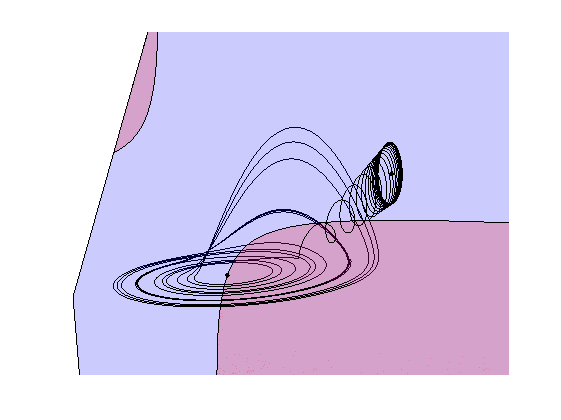
\includegraphics[width=0.30\textwidth,clip=true]{RoessNearEq}
\end{center}
  \caption{\label{fig:RoessNearEq}
  A R\"ossler flow Poincar\'e section $\PoincS_{-}$ through the inner
  {\eqv} $\ssp_{-}$ and its stable eigenvector.
}
\end{figure}
%%%%%%%%%%%%%%%%%%%%%%%%%%%%%%%%%%%%%%%%%%%%%%%%%%%%%%%%%%%%%%%%%%%%%

%%%%%%%%%%%%%%%%%%%%%%%%%%%%%%%%%%%%%%%%%%%%%%%%%%%%%%%%%%%%%%%%%%%%%
\begin{figure}%[H]
\begin{center}
  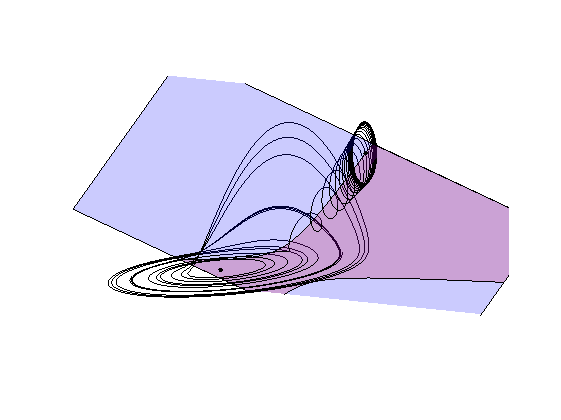
\includegraphics[width=0.30\textwidth,clip=true]{RoessFarEq}
\end{center}
  \caption[R\"ossler section, outer {\eqv}]{
  A Poincar\'e section for R\"ossler flow
      through the
      outer
  {\eqv} $\ssp_{+}$  and its unstable eigenvector.
  } \label{fig:RoessFarEq}
\end{figure}
%%%%%%%%%%%%%%%%%%%%%%%%%%%%%%%%%%%%%%%%%%%%%%%%%%%%%%%%%%%%%%%%%%%%%

%%%%%%%%%%%%%%%%%%%%%%%%%%%%%%%%%%%%%%%%%%%%%%%%%%%%%%%%%%%%%%%%%%%%%
\begin{figure}%[H]
\begin{center}
  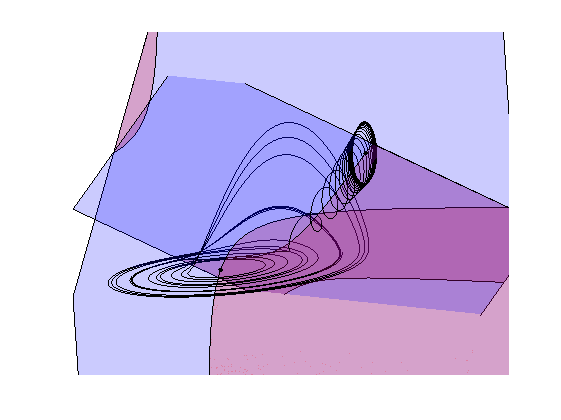
\includegraphics[width=0.30\textwidth,clip=true]{RoessBothEq}
\end{center}
  \caption{
  A two-section atlas for R\"ossler flow, with the local sections of
  \reffigs{fig:RoessNearEq}{fig:RoessFarEq} oriented and combined so that
  the ridge (intersection of the two sections, indicated by the brown
  line in individual sections) lies  approximately midway between the
  \template s.
  } \label{fig:RoessBothEq}
\end{figure}
%%%%%%%%%%%%%%%%%%%%%%%%%%%%%%%%%%%%%%%%%%%%%%%%%%%%%%%%%%%%%%%%%%%%%

    \ifdraft\color{blue}

For R\"ossler flow \refeq{eq:Rossler}
[blah blah]
%\subsection{R\"ossler two-chart atlas}

The point is that while it is impossible to visualize  $(d\!-\!2)$\dmn\
{\poincBord}, a trajectory crossing can be determined by a simple linear
check, and easy to visualize in any dimension.

% \subsection{$N$-chart atlas, forward maps}
% \subsection{Ring of Fire return map\rf{lanCvit07}}

The two charts
\reffigs{fig:RoessNearEq}{fig:RoessFarEq} illustrate \poincBord,
and \reffigs{fig:RoessBothEq} the combined 2-chart atlas.

    \color{black}\fi

A Poincar\'e section is {\em not} a projection onto a lower-dimensional
space: Rather, it is a local change of coordinates to a direction along
the flow, and the remaining coordinates transverse
to it. No information about the flow is lost; the full space trajectory
can always be reconstructed by integration from a point in the
section.

Finally, we note that the method of Poincar\'e sections is {not}
equivalent to \emph{strobing} a flow at a sequence of instants in time.
While `strobing' is what any numerical integrator does, by representing a
trajectory by a sequence of time-integration step separated points,
strobing is in general not a reduction of a flow, as the sequence of
strobed points still resides in the full \statesp\ $\pS$, of
dimensionality $d$.

    \ifdraft\color{blue}
\subsection{\Statesp\ visualization}

On perils of thinking linearly: bases such as Fourier modes are
perfectly natural for problems such a bifurcation of a steady state, and
other weak perturbations. They are absolutely unnatural for strongly
nonlinear problems, with many Fourier modes of comparable magnitude and
strongly entangled.

        There is always tension between mathematics - linear problem eigenmodes
        (Fourier for translations and rotations) and physics - the fact that
        nonlinear dynamics states are far away from such axes, as they
        always involve a number of such linear modes strongly entangled.

\subsection{Time orbit: point is a point, line is a line in all dimensions}
\label{sect:TimeOrb}


    \color{black}\fi
